\chapter{Hauptteil}
%

% Bis 3.1 kann weg: wurde nur zum reinkommen geschrieben

Um ein grundlegendes Verständnis für die Analyse von Dateiformaten zu entwickeln wird einem klaren Schema gefolgt. Mit diesem Schema wird sich an der chronologischen Reihenfolge von der Entstehung eines Tons bis zur Verarbeitung im Code orientiert.

\par

Jeder Ton wird durch eine Vibration erzeugt. Diese Vibration kann durch unterschiedliche Gegenstände erzeugt werden. Dazu zählen Becken eines Schlagzeugs, Saiten eines Basses oder die Stimmbänder (?).

%
\begin{enumerate}
    \item Was ist ein Ton
    \item Formen der Musikdarstellung
    \item Darstellung in der Mathematik
    \item Vorstellung Fourier Transform
    \item Ton und Fourier als Code
    \item Trennung von Instrumenten im Code
    \item Vorgehen im Projekt (evtl früher)
    \item Wie kann man auf dem Stand aufbauen? (/Wie könnte es weitergehen?)
    \item Fazit
    \begin{enumerate}
        \item Aufwand
        \item Ertrag (z.B. erworbenes Wissen)
    \end{enumerate}
\end{enumerate}
%

%
(Bis hier muss überarbeitet werden?)
%

%
\section{Formen der Musikdarstellungen}
%

%
(Einleitung und Überschriften?)
%

Musik kann unterschiedlich dargestellt werden. Je nach Bedarf, wird eine andere Form der Musikdarstellung benötigt. Eine Form der visuellen Musikdarstellung sind Musiknoten. Es ist eine formale Sprache, die vorgibt wie ein Musikstück gespielt wird \parencite{sheet_music_representations}.

\par

 - MIDI nutzt Notendarstllung

\par

Eine weitere Form der Darstellung, ist die Audiodarstellung. In diesen Darstellungen werden alle Informationen der Töne als Audiosignale digital gespeichert und geteilt. Dazu gehören auch das Timing, die Intensität, die Lautstärke, die Länge des Tons und vieles mehr. Es werden nicht die einzelnen Töne und Noten gespeichert, sondern die Frequenzen während der Aufnahme in Abhängigkeit zur Zeit. Die Audiodatei kann auch Nebengeräusche oder weitere Instrumente beihalten.

\par

Das macht es schwieriger unterschiedliche Audiosignale zu trennen und die ursprünglichen Noten (Töne?) wieder herzustellen. Die verbreitetste Form der Audiodarstellung ist MP3 (Quelle?). In diesem Projekt werden jedoch Wave Dateien behandelt. Die Unterschiede, sowie Vor- und Nachteile der Audiodarstellungen werden in (...?) behandelt \parencite{fundamentals_of_music_processing} (Kapitel?).

 - Musik Darstellung in Audiodateien
 - Was ist eine Note audio-/ visuell

%
\section{Was ist ein Ton?}
%

Töne entstehen durch die Vibration eines Gegenstandes. Diese erzeugen Schallwellen. Der Luftdruck einer Schallwelle wird graphisch als eine Sinus- oder Cosinusfunktion dargestellt.

%
(Bild?)
%

 - Was sind Frequenzen Lautstärke etc. (Stauchung/ Streckung..., Verlauf)
 - Frequenz bei 4 Perioden/ Maxima in einer Sekunde -> 4Hz?
 - "The sinusoid can be considered the prototype of an acoustic realization of a musical note. Sometimes the sound resulting from a sinusoid is called a harmonic sound
or pure tone"

%
\section{Aufbau einer Audiodatei/ Music Representation}
%

Für die Aufnahme von Audiosignalen werden analoge Signale in eine digitale Form von Schall umgewandelt. Die analoge Signaldarstellung verwendet kontinuierliche und konstante Spannungsschwankungen, die den verursachten Luftdruckschwankungen entsprechen \parencite{digital_representation}. In der digitalen Form werden die Spannungsschwankungen als Bitstreams gespeichert und je nach Audio-Format komprimiert.

%
 - Noten sind ebenfalls musikalische Darstellung
 - Entstehung der Audiosignale: Analog/ Digital
 %

%
\subsection{Durchführung der Komprimierung}
%

Die Komprimierung von Audiodateien wird meistens verwendet, um mehr Musik auf einem Datenträger speichern zu können \parencite{what_is_audio_compression}. Um eine Aufnahme zu komprimieren wird diese in eine Sampling Rate und eine Quantisierungsgröße reduziert.

\par

%
\textbf{Sampling Rate}
%

Die Sampling Rate (/Sampling-Rate?) definiert (/beschreibt?) die Anzahl von gespeicherten Signalen pro Sekunde. Dies reduziert die benötigten gespeicherten Daten von einer durchgängigen Aufnahme auf mehrere Blöcke. Beispielsweise hat eine CD Aufnahme eine Sampling Rate von 44.100 Samples pro Sekunde (kurz: 44.1 kHz), das heißt es werden 44.100 Soundsignale pro Sekunde gespeichert, dessen Übergänge kaum wahrnehmbar sind, jedoch bereits zu einem deutlichen Reduzierung des Speicherbedarfs führen.

%
(Bild einfügen?)
%

%
\textbf{Quantisierungsgröße (deutscher Fachbegriff?)}
%

Die Quantisierungsgröße beschreibt die Komprimierung pro Sample. Die möglichen Werte eines Samples sind fließend (Fachbegriff für Einheiten mit unendlich Nachkommastellen?) und werden mit der Quantisierungsgröße eingegrenzt. Damit wird die Anzahl der möglichen Werte eingegrenzt und dessen Unterschied festgelegt. Beispielsweise wird bei CDs ein 16-bit coding scheme (Deutsch?) gewählt, welches 65.536 mögliche Werte festlegt.

%
(Bild einfügen?)
%

%
\subsection{Waveform Audio File Format}
%

Waveform Audio File Format (kurz: WAV) sind Dateien, die Audioaufnahmen unkomprimiert speichern \parencite{what_is_a_wav_file}. Es wird \enquote{vom englischen Wort \enquote{wave} abgeleitet, und steht in diesem Zusammenhang für Schallwelle} \parencite{wav}. Für die in diesem Projekt behandelte (Fast?) Fourier Transformation sind die Höhe der \enquote{Abtastrate fs des Messsystems} und die Quantitätsgröße (siehe Kapitel...?) bedeutsam \parencite{FFT_grundlagen}. Durch die unkomprimierte Form (ist die Abtastrate (/Quantitätsgröße?) hoch und) kann die Trennung von Tonspuren (Referenz?) durchgeführt werden.


%
\subsection{Andere Formen von Audio-Dateien}
%

%
\begin{itemize}
    \item MP3
    \item WMA
    \item AAC
    \item OGG
    \item FLAC
    \item RM
\end{itemize}
%

\parencite{audioformate_im_überblick}

%
\section{Trennung einer Tonspur in verschiedene Instrumente}
%

Eine Aufnahme speichert aufgenommene Signal in Abhängigkeit zur Zeit. Jedes der eingehenden Signale verfügt über Schwingungen in Form von einer Amplitude. Bei einer Aufnahme vermischen sich die verschiedenen Signale zu einer Amplitude und sind schwierig zu differenzieren. Beispielsweise von Hintergrundgeräuschen oder bei der Aufnahme mehrer Musikinstrumente. Die Trennung von Instrumenten einer Tonspur wird in Forschung und Bildung behandelt (Quelle?). Die verbreitetste (Quelle?) Vorgehensweise ist die Verwendung der Fourier Transformation (Gibt es andere Vorgehensweisen?).

%
\subsection{Fourier Transformation}
%

Die Fourier Transformation ist ein Algorithmus der die Darstellung einer Tondatei verändert. Ursprünglich liegt die Audiospur mit einer Kombination aus unterschiedlichen Frequenzen in Abhängigkeit zur Zeit vor. In dieser Darstellung sind die unterschiedlichen Signale schwierig zu trennen und wird von der Fourier Transformation transformiert.

\par

%
\subsubsection{Entwicklung der Fourier Transformation}
%

Die Fourier-Transformation ist eine Generalisierung der Fourierreihen. Diese können (stetige?) Funktionen in mehrere Funktionenreihen aufteilen. Bereits im 18. Jahrhundert wurden Fourierreihen für einzelne Funktionen entdeckt. Im Jahr 1822 behauptete Joseph Fourier, dass Funktionenreihen für jede Funktion existieren. Erst im 20. Jahrhundert wurden Funktionenreihen für die übrigen stetigen oder stückweise stetigen Funktionen entdeckt. Durch die Vollständigkeiten der Funktionenreihe kann die Transformation auf jegliche Funktionen (welche Funktionen?) angewendet werden und wurde nach Fourier benannt.

\par

\subsubsection{Durchführung der Transformation}

Die Fourier Transformation ist ein mathematisches (?) Vorgehen, indem die zeitliche Darstellung in eine frequentielle Darstellung transformiert wird. Die Transformation ermöglicht es jegliche Funktionen in eine Summe aus Sinus und Kosinus Wellen unterschiedlicher Frequenzen zu zerlegen.

\par

 - Vergleichsschwingungen
 
\par

In der neuen Darstellung werden die Frequenzen der Funktion unabhängig von der zeitlichen Komponente wiedergegeben. Unterschiedliche Frequenzen können unterschiedlichen Signalen zugeordnet werden. Die frequentielle Darstellung gibt an welche Signale in welchen Frequenzen Teil der Funktion sind, allerdings nicht wann. Daher wird die Darstellung wieder umgeformt in die zeitliche Abhängigkeit. 

\par

Das Signal oder die Signale, die von der Tonspur getrennt werden, können in der frequentiellen Darstellung identifiziert werden. Anschließend werden diese von den übrigen Signalen getrennt und zurück in die ursprüngliche Darstellung transformiert. Damit erhält man eine neue Tondatei, die ausschließlich aus den benötigten Signalen besteht.

\par

Anschließend werden die Tonspuren je nach Frequenz extrahiert und der Vorgang wieder rückgängig gemacht. Somit liegen diese als WAV-Datei vor und können weiterverwendet werden.

%
(Bild?)
%

\subsubsection{Parameter der Transformation}

 - Probleme:
    - Rechenaufwand/ Dauer

In (...?) wurden die Samples und Quantisierungsgrößen behandelt, die für die Durchführbarkeit der Transformation relevant sind. Zudem können Komponenten bei der Durchführung (Synonym?) parametrisiert werden.

\par

%
\textbf{Blocklänge (/engl.?)}
%

Ein Parameter für die Durchführung der Fourier-Transformation ist die Blocklänge (kurz: BL). Diese behandelt die Anzahl an Samples die bei der Fourier-Transformation betrachtet werden. 

\par

Umso länger die BL, desto präziser wird die Transformation durchgeführt. Jedoch bedeutet dies auch mehr Rechenaufwand und eine längere Dauer der Transformation. Bei einigen Anwendungsszenarien führt dies zu einer Abwägung zwischen Dauer und Genauigkeit der Durchführung. Beispielsweise bei einer App zum stimmen von Instrumenten und erkennen der gespielten Töne (Quelle?).

\par

\subsubsection{Durchführung am Beispiel einer Musiknote}

In diesem Beispiel (Müller referenzieren?) wird eine Note auf einem Piano gespielt und durch die Transformation in eine frequentielle Darstellung der gespielte Ton erkannt.

\par

Die Aufnahme des Tons ist in \cref{fig:fourier}(a) zu erkennen. Für die Transformation wird ein Ausschnitt von 10ms verwendet. Das entspricht der Blocklänge und reduziert den Rechenaufwand (referenzieren?).

\par

Anschließend werden unterschiedliche Vergleichsfunktion für die jeweiligen Frequenzen mit dem Ausschnitt der Tonspur verglichen. Die Ähnlichkeiten der jeweiligen Frequenzen werden in (f) wiedergegeben.

\par

In \cref{fig:fourier}(c) ist die Übereinstimmung für die Frequenz w = 262 Hz besonders hoch. Daraus folgt in (f) bei ungefähr 262 der höchste Wert. Die Höhe des Wertes wird in der Variable dw angegeben.

% w = ω

\par

Die Frequenz 262 entspricht der Note C4. Darüberhinaus wird bei einer Frequenz von 523 (siehe \cref{fig:fourier}(d)) eine hohe Übereinstimmung erkannt. Dies entspricht ungefähr der Frequenz des zweiten Teils der Note C4 (zweiter Teil?).

%
 - anschließend trennen?
%

%
\begin{figure}
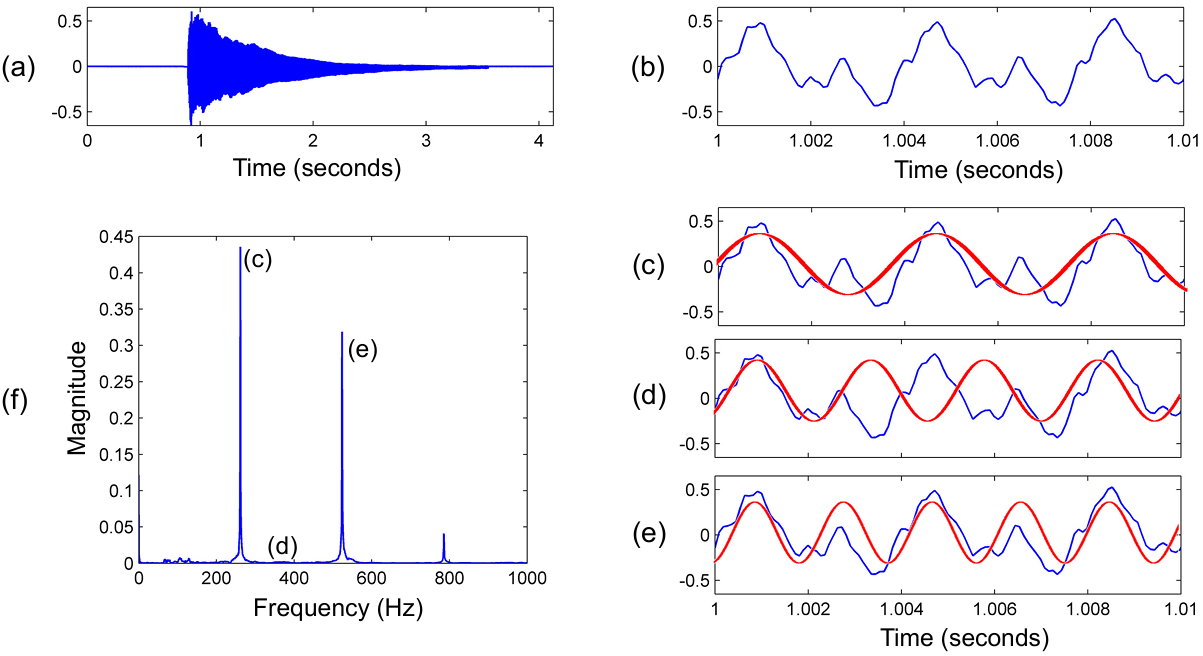
\includegraphics[width=1\textwidth]{images/Fourier_math.PNG}
\caption{Note C4 in unterschiedlichen Darstellungen}
\label{fig:fourier}
\end{figure}
% Music Processing S.41
%

%
\textbf{Nachteile}
%
    
Die Fourier Transformation ermöglicht es je nach Bedarf zwischen der zeitlichen oder der sequentiellen Darstellung zu wechseln. Allerdings ist bei der Fourier Transformation der Wechsel zwischen den Darstellung notwendig und es wird entweder die zeitliche oder die frequentielle Komponente ignoriert. Bei der Anwendung der Fourier Transformation gibt es keine Darstellung die beide Komponente kombiniert.

    - Darstellung (nie Zeit und Frequenz)

(Noch unklar wie unterschiedliche Instrumente vorliegen, aber analoge Instrumente sollten in Sinusfunktion vorliegen und erkennbar sein)

%
\subsection{Wavelet-Transformation}
%

Die Wavelet-Transformation ist ein Vorgehen, das eine Funktion der zeitlichen Darstellung in eine 3(-?)dimensionale Darstellung in Abhhängigkeit von Zeit und Frequenz erstellt. Dafür werden Wellenfunktionen mit der ursprünglichen Funktion auf Übereinstimmungen verglichen. Es Wellenfunktionen gibt unterschiedliche Wellenfunktionen und sie werden Wevelets genannt. Der Name ist aus dem französichen und wird in kleine Welle oder Wellchen übersetzt.

\par

Im Gegensatz zu der ursprünglichen Funktion sind die Flächen der Wavelets endlich und daher der Name (finite energy). Eine weitere Bedingung für Wavelets ist, dass das Integral null ergibt. Also die Fläche über und unter der X-Achse gleichgroß ist (Admissibility condition). Jede Wavelet wird um die Parameter m und b ergänzt.

%
\begin{itemize}
    \item[m:] Bestimmt die Frequenz der Wavelet
    \item[b:] Bestimmt den Zeitpunkt der Wavelet
\end{itemize}
%

Zudem hat die Wavelet einen realen und einen imaginären Teil. Das bedeutet, dass durch die Ergänzung der imaginären Zahl die Wavelet um eine Achse ergänzt wird und 3(-?)dimensional wird. Sowohl der reale als auch der imaginäre Teil der Wavelet werden mit der Funktionen verglichen und durch die Multiplikation (Begriff?) erhält man die Ähnlichkeit der Funktion und der Wavelet.

\par

Die Ähnlichkeit der Wavelet mit der Funktion wird für jedes m und b berechnet und in dem 3-dimensionalen Ausgabe-Graphen in Abhängigkeit zur Zeit angegeben. Dies hat den Vorteil das man eine Darstellung des Signals in Abhängigkeit von Zeit und Frequenz erstellen kann.

\par

Dies kann beispielsweise sinnvoll in der Überprüfung von Ampelleuchten sein. Während die Fourier-Transformation die unterschiedlichen Frequenzen der Farben grün, gelb und rot erkennt und wiedergibt ob die drei Lichter leuchten, kann die Wavelet-Transformation angeben, ob die Lampen jeweils zum richtigen Zeitpunkt leuchten \parencite{wavelets}.

%
 - verwendet spezialisierte Funktionen: Wavelets
 - aus französisch Wellchen/ kleine Welle
 - Familie an Funktionen
   - jede für spezielle Anwendung
 - Integral unter und über X-Achse gleichgroß
   - Admissibility condition
 - endliche Fläche
   - finite energy
   - lokalisiert in Zeit